% ============================================================
\chapter{マクロ経済とボラティリティ}\label{ch:macro}

金利、インフレ、景気の局面などのマクロ経済の情報は、資産クラスの期待リターンとリスクの両方に効く。BL では、マクロの情報を (1) 時系列モデルの予想としてビュー $Q$ に入れる、(2) ボラティリティの予想として $\Omega$ や $\Sigma$ に入れる、という 2 通りに使える。この章では、ボラティリティのモデル（GARCH の仲間）を使う研究を読み、本プロジェクトのデータで EGARCH-M を推定して、両方の使い方を試す。

\section{研究の例}

\begin{paperbox}[Beach and Orlov（2007）, \textit{An application of the Black--Litterman model with EGARCH-M-derived views for international portfolio management}, Financial Markets and Portfolio Management 21(2)]
\begin{itemize}
\item BL を世界の株式の配分に当てはめる。新しい点は、GARCH の仲間のモデル（EGARCH-M）から作ったビューを BL の入力にすることである。
\item このポートフォリオは、市場の均衡の比率や、Markowitz の最適な比率に基づくポートフォリオより高いリターンを上げた。
\end{itemize}
本文は確認できず、要旨の範囲で記した。調査メモは、この論文の平均の式（マクロ変数を含む）、1 期先の条件付き分散をそのまま $\Omega$ の対角にすること、$\tau$ を 0.005 と 0.01 にしたことを書いているが、この資料では確認できなかった。
\end{paperbox}

\begin{paperbox}[Duqi, Franci and Torluccio（2014）, \textit{The Black--Litterman model: the definition of views based on volatility forecasts}, Applied Financial Economics 24(19)]
\begin{itemize}
\item EGARCH-M でボラティリティを予想し、その予想をビューを決める入力にする。
\item 株価のリターンの時系列に見られる経験的な規則性と、運用者のその規則性への見方を組み合わせることを目指す。
\item EGARCH に基づく入力で、かなりの利点がありうる配分が得られた、と述べている（要旨の範囲）。
\end{itemize}
\end{paperbox}

\begin{paperbox}[Sun, Wu and De（2023）, \textit{A Novel Black-Litterman Model with Time-Varying Covariance for Optimal Asset Allocation of Pension Funds}, Mathematics 11(6)]
\begin{itemize}
\item 年金の資産配分は長期の問題なので、長期のリスクとリターンの見込みが要る。長期の共分散は推定が難しい（データが少ない、短期の共分散を積み上げると変化を取りこぼす）。
\item 資産のリターンを VARMA、共分散を GARCH でモデル化し、短期の共分散を長期の見込みに直して BL に使う（TVC-BL）。
\item 従来の BL と比べ、リスク回避度 1、1.5、3 で、シャープレシオがそれぞれ 13.0\%、10.5\%、12.8\% 高かった。
\end{itemize}
\end{paperbox}

\chapref{ch:politics} の Han と Li（2023）も、GARCH-MIDAS で政策の不確実性に応じたボラティリティを作り、ビューの不確かさに使う研究である。Teplova ほか（2023）は、ARMA-GARCH とコピュラから作った期待リターンをビューにしている（\chapref{ch:cop}）。

\section{EGARCH-M}

EGARCH（Nelson 1991）は、分散の対数をモデル化するので、分散が負にならず、下落と上昇で反応が違う（下落のあとにボラティリティが大きく上がる）ことを表せる。平均の式に条件付きの標準偏差を入れたものが EGARCH-M（M は in-Mean、Engle、Lilien、Robins 1987 の ARCH-M の考え方）である。この資料では次の形を使う。
\begin{align}
r_t&=c+\gamma\,\sigma_t+\varepsilon_t,\qquad \varepsilon_t=\sigma_tz_t,\quad z_t\sim\mathcal N(0,1)\label{eq:egarch-mean}\\
\log\sigma_t^2&=\omega+\beta\log\sigma_{t-1}^2+\alpha\bigl(|z_{t-1}|-\E|z|\bigr)+\xi z_{t-1}\label{eq:egarch-var}
\end{align}
$\gamma$ はリスクの見返り（リスクが高いほど期待リターンが高いか）、$\alpha$ はショックの大きさへの反応、$\xi$ は向きへの反応（負なら下落で分散が大きく上がる）、$\beta$ は持続性である。平均の式に何を入れるか（$\sigma_t$、$\sigma_t^2$、$\log\sigma_t^2$）や、マクロ変数を入れるかは、研究によって違う。

\subsection*{\SP{} の日次リターンで推定する}

本プロジェクトの DB の \SP{} の日次の超過リターン（13 週の財務省証券の利回りを引く、パーセント表示）で、\V{eg.start}〜\V{eg.end} の \V{eg.n} 日について、正規分布の最尤法で推定した。

\begin{table}[htbp]
\centering
\caption{EGARCH-M の推定値（\SP{} の日次超過リターン、\%）。標準誤差は対数尤度の数値の 2 階微分から。対数尤度は \V{eg.ll}。}
\label{tab:egarch}
\tabin{egarch}
\end{table}

\begin{figure}[htbp]
\centering
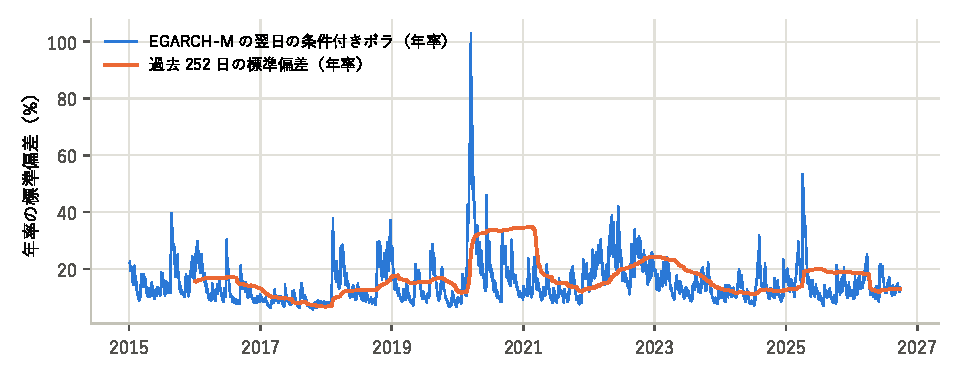
\includegraphics[width=0.95\linewidth]{fig_egarch_vol.pdf}
\caption{EGARCH-M の翌日の条件付きボラティリティ（年率）と、過去 252 日の標準偏差（年率）。}
\label{fig:egarch-vol}
\end{figure}

\tabref{tab:egarch} から分かることを挙げる。

\begin{itemize}
\item 向きへの反応 $\xi=\V{eg.xi}$ は、$t$ 値で $-8$ 程度とはっきり負である。下落の日のあとに、ボラティリティが大きく上がる。
\item 持続性 $\beta=\V{eg.beta}$。ボラティリティの高い状態はしばらく続くが、数週間で戻る。
\item リスクの見返り $\gamma=\V{eg.gamma}$ の $t$ 値は \V{eg.gamma.t} で、0 と区別できない。
\end{itemize}

\figref{fig:egarch-vol} の条件付きボラティリティは、\V{eg.argmax} に年率 \V{eg.max}\% まで上がった。過去 252 日の標準偏差は、その動きにかなり遅れてついていく。

\section{平均の式をそのままビューにすると}

EGARCH-M の平均の式~\eqref{eq:egarch-mean} は、翌日の期待リターン $c+\gamma\sigma_{t+1}$ を出す。これを 21 倍して翌月の予想にすると、中央値は \V{eg.mu.med}\% だが、最小 \V{eg.mu.min}\%、最大 \V{eg.mu.max}\% と、ボラティリティが高い時期に極端に大きくなる。$\gamma>0$ の推定値のもとでは、「危ないときほど期待リターンが高い」という予想になるからである。

これは理屈としては「リスクの高いときにはリスクプレミアムが高い」を表しているが、$\gamma$ は有意でなく、推定の誤差が大きい。このまま BL のビューにすると、危機のさなかに強い強気のビューを置くことになる。マクロのモデルの平均の式からビューを作るときは、

\begin{itemize}
\item 平均の式の係数が有意かを確かめる。有意でなければ、平均の予想は使わない（均衡のまま）。
\item 予想が過去の範囲から大きく外れる時期は、ビューを入れないか、上限を置く。
\item 予想の当たり具合（IC、較正の傾き）を、過去のデータで確かめてから採用率を決める（\chapref{ch:accuracy}）。
\end{itemize}

ことが必要である。

\section{条件付き分散で $\Omega$ を決める}

調査メモは、EGARCH-M の 1 期先の条件付き分散を $\Omega$ の対角にすれば、ボラティリティが急に上がる局面では自動的にビューの確信が下がり、均衡のほうへ戻る「自己修復」の仕組みになる、と述べている。この考え方を確かめる。

採用率は、$\Omega$ と $\tau\Sigma$ の比で決まる。$\Omega$ を条件付き分散 $\sigma_{t+1|t}^2$ に比例させ、$\tau\Sigma$ を過去 252 日の分散 $v_{252,t}$ に比例させると、比例の定数をそろえたとき、採用率は
\begin{equation}
s_t=\frac{v_{252,t}}{v_{252,t}+\sigma^2_{t+1|t}}
\end{equation}
となる。ふだん（2 つが同じくらい）は 50\% である。

\begin{figure}[htbp]
\centering
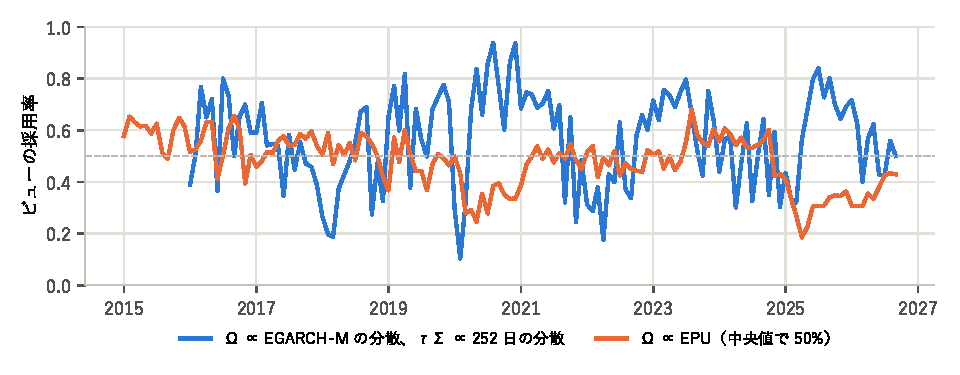
\includegraphics[width=0.95\linewidth]{fig_adoption_time.pdf}
\caption{$\Omega$ をボラティリティの見込みで伸び縮みさせたときの採用率（月末）。青は EGARCH-M の条件付き分散と過去 252 日の分散の比、橙は EPU の水準（中央値で 50\%）。}
\label{fig:adoption-time}
\end{figure}

\figref{fig:adoption-time} の青の線は、次のことを示している。

\begin{itemize}
\item ボラティリティが急に上がった 2020 年 2 月末には、条件付き分散が過去 252 日の分散をはるかに上回り、採用率は \V{eg.adopt.min}\% まで下がった。調査メモの言う「自己修復」である。
\item ところが、危機のあとの 2020 年 8 月には、過去 252 日の分散に危機の時期が含まれる一方で、条件付き分散は下がっているため、採用率は \V{eg.adopt.max}\% まで上がった。危機が去った直後に、ビューをいちばん強く信じる設定になる。
\end{itemize}

採用率の動きは、$\Omega$ と $\Sigma$ を「どれだけ速く動かすか」の差から生まれている。$\Sigma$ も GARCH のような速い見込みで動かせば、2 つは同じように動き、採用率はほとんど変わらない。逆に、$\Sigma$ を長い期間で推定したまま $\Omega$ だけを速く動かすと、危機の始まりでビューを捨て、危機の直後にビューを強く信じることになる。

これが望ましいかどうかは、ビューの当たり具合が局面でどう変わるかによる。危機の直後に予想が当たりやすいという根拠がなければ、意図しない動きである。

\begin{tipbox}[コツ：ボラティリティで $\Omega$ を動かすとき]
\begin{enumerate}
\item 採用率を動かしているのは $\Omega$ と $\tau\Sigma$ の比である。$\Omega$ だけを動かすと、$\Sigma$ との速さの違いがそのまま採用率の動きになる。
\item 「ボラティリティが高いときは予想が外れやすい」だけなら、$\Omega$ と $\Sigma$ を同じ速さで動かすので十分である。採用率は変わらず、比率の傾きはリスクに応じて小さくなる。
\item 「ボラティリティが高いときは、予想の当たり具合（IC）そのものが下がる」と考えるなら、それを過去のデータで確かめ、IC の変化として採用率に入れる。
\end{enumerate}
\end{tipbox}

\section{景気の局面のビュー}

調査メモは、景気循環の局面（拡大、後退など）を特定し、その局面での各資産クラスの過去の平均超過リターンをビューにし、CVaR を最小にする最適化と組み合わせた「CVaR-BL-MCV」というモデルが、年金の配分でシャープレシオを平均 19.7\% 改善した、と紹介している。この資料では、この名前のモデルと数字を述べた論文を見つけられなかった（\appref{app:check}）。近い研究として、上の Sun・Wu・De（2023）の TVC-BL（シャープレシオが 10.5〜13.0\% 改善）と、CVaR を使う BL の研究（\chapref{ch:cop}、\chapref{ch:cvar}）がある。

局面のビューを作るときの一般的な注意を挙げる。

\begin{itemize}
\item \textbf{局面の数が少ない}：アメリカの景気後退は、戦後で十数回しかない。局面ごとの平均リターンは、少ない例の平均で、誤差が大きい。$\Omega$ はその誤差に見合う大きさにする。
\item \textbf{局面の判定の先読み}：景気後退の公式の日付（NBER）は、数か月から 1 年以上あとに発表される。過去の検証で公式の日付を使うと、その時点では分からなかった情報を使うことになる。判定には、その時点で手に入ったデータだけを使う。
\item \textbf{局面の確率}：局面がはっきりしない時期は、局面ごとのビューを確率で重み付けし、局面の不確かさも $\Omega$ に入れる。
\end{itemize}

\section{マクロのファクターモデル}

マクロの変数をファクターとして使い、ファクターへのビューを置く方法もある（\chapref{ch:shape}）。Chen、Roll、Ross（1986）は、鉱工業生産、インフレの予想外の変化、長短金利差、信用スプレッドなどが、株式のリターンに価格付けされたファクターであることを示した。「景気が予想より強い」というビューを鉱工業生産のファクターに置けば、各資産への影響は露出を通じて一貫した形で決まる。ファクターのプレミアムの事前分布と当たり具合を、長いデータで測れるのも利点である。

\begin{keybox}[この章のまとめ]
\begin{itemize}
\item マクロのモデルは、平均の予想（$Q$）とボラティリティの予想（$\Omega$、$\Sigma$）の両方に使える。
\item \SP{} の EGARCH-M では、下落への非対称な反応ははっきりしていたが、リスクの見返り $\gamma$ は有意でなかった。平均の式をビューにすると、危機の時期に極端な強気になる。
\item 条件付き分散で $\Omega$ だけを動かすと、危機の始まりに採用率が \V{eg.adopt.min}\% まで下がる一方、危機の直後に \V{eg.adopt.max}\% まで上がる。$\Omega$ と $\Sigma$ の速さをそろえるかどうかを意識して決める。
\item 景気の局面のビューは、局面の数の少なさと、判定の先読みに注意する。
\end{itemize}
\end{keybox}
